%  Document History:
%
%-----------------------------------------------------------------------
\documentclass[a4paper,oneside]{arlimsTPPM}
%------------------------------------------------------------------------- 

%--- Settings for the ARLIMS document class ---
%\setcounter{page}{8} % The starting page

%--- This part of the preamble can be fiddled with according to our needs ---

% Some packages that we like and want to use:
\usepackage{cite}
\usepackage{url}
\usepackage{graphicx}
\usepackage{color}
\usepackage[T1]{fontenc}
\usepackage[scaled]{beramono}

% For typesetting listings.
\usepackage{listings}
\lstset{% Set some listing parameters.
  numbers=left,
  numberstyle=\sffamily\scriptsize,
  numberblanklines=false,
  basicstyle=\ttfamily\footnotesize,
  showstringspaces=false,
  backgroundcolor=\color[rgb]{0.9,0.9,0.9},
  %frame=tb,
  %xleftmargin=4.3ex,
  language=Python
}
\usepackage{hyperref}

% The path(s) to the graphics files:
\graphicspath{{eps/}{pdf/}}

% correct bad hyphenation here
%\hyphenation{cor-res-pon-ding net-works}

% This makes line breaks look prettier
\sloppy

% Conventions for typesetting vectors and matrices.
\renewcommand{\vec}[1]{\boldsymbol{#1}}
\newcommand{\mat}[1]{\boldsymbol{#1}}
% If \boldsymbol doesn't work, try \pmb (poor man's bold, which
% "multistrikes" every letter with small offsets.

%--- Preamble definitions for actual content ---

\title{An Introduction to pulp for Python Programmers}
\author{Stuart Mitchell}

\institute{
\begin{minipage}[t]{.45\textwidth}\centering
Light Metals Research Centre\\
University of Auckland\\
Auckland, New Zealand\\
\textnormal{\texttt{\small s.mitchell@auckland.ac.nz}}
\end{minipage}}



%------------------------------------------------------------------------- 
\begin{document}

% Put a proper title on the first page:
\maketitle

%------------------------------------------------------------------------- 
\begin{abstract}
  Pulp-or (referred to as pulp for the rest of this paper) is a linear programming framework in Python. Pulp is licensed under a modified BSD license. The aim of pulp is to allow an Operations Research (OR) practitioner or programmer to express Linear Programming (LP), and Integer Programming (IP) models in python in a way similar to the conventional mathematical notation. Pulp 
  will also solve these problems using a variety of free and non-free LP solvers. Pulp models an LP in a natural and pythonic manner.
This paper is aimed at the python programmer who may wish to use pulp in their code. As such this paper contains a short introduction to LP models and their uses.

  % ARLIMS style
  \paragraph{Keywords:} Linear programming; Operations Research; pulp-or.
\end{abstract}

%------------------------------------------------------------------------- 
\section{Introduction}

Operations Research is known by the catch phrase ``The science of better''. From the website \cite{scienceofbetter} we find this brief description

\begin{quote}
In a nutshell, operations research (O.R.) is the discipline of applying advanced analytical methods to help make better decisions. 
\end{quote}

The particular area of operations research where pulp is useful is the development and modelling of Linear Programming (LP) and Integer Programming (IP) problems. Mathematically, an LP problem is to find a point in a n-dimensional linearly constrained region that maximises a given linear objective function. IP is an LP where the solution must contain discrete variables which take an integer value at the solution, a common special case of an integer variable is a binary variable which must be either 0 or 1 at the solution.

In general terms, an LP can describe a problem were decisions must be made (for example, the quantity of each ingredient in a can of cat food, detailed in section \ref{sec:whiskas}). These decisions are constrained by the properties of the problem that they model (the total weight of ingredients must be 100 grams and dietary requirements must be met). The quality of a solution is determined by some sort of cost (the total dollar cost to produce the can) and you seek to minimise or maximise the cost subject to the constraints.



\section{A Brief introduction to Linear Programming}
\label{sect:LP}

In this section we will introduce the reader to the structure of an LP problem and show the syntax used to formulate these models in pulp. The following is a example LP motivated by a real-world case-study. In general, problems of this sort are called `diet' or `blending' problems. An extensive set of case studies (including those below) can be found in \cite{pulpwiki}.

\subsection{The Whiskas Cat Food Problem (whiskas.py)}
\label{sec:whiskas}

\begin{figure}[h]
 \centering
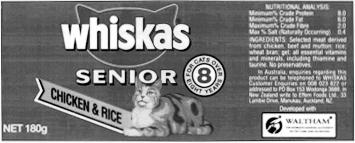
\includegraphics{images/whiskas_label.jpg} 
\caption{A Whiskas cat food label.}
\end{figure}
Whiskas cat food, shown above, is manufactured by Uncle Ben's. Uncle Ben's want to produce their cat food products as cheaply as possible while ensuring they meet the stated nutritional analysis requirements shown on the cans. Thus they want to vary the quantities of each ingredient used (the main ingredients being chicken, beef, mutton, rice, wheat and gel) while still meeting their nutritional standards. 

\begin{figure}[h]
 \centering
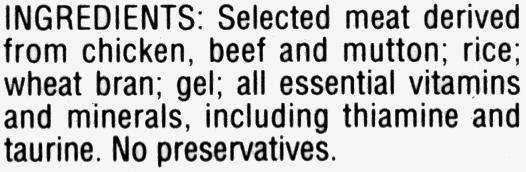
\includegraphics[scale=0.5]{images/whiskas_ingredients.jpg}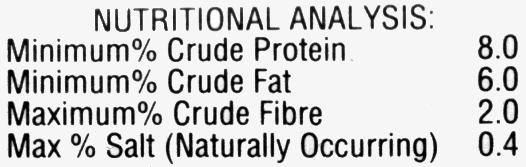
\includegraphics[scale=0.5]{images/whiskas_nutrition.jpg}
\caption{Detail of ingredients and nutritional requirements.}
\end{figure}

\begin{figure}[h]
 \centering
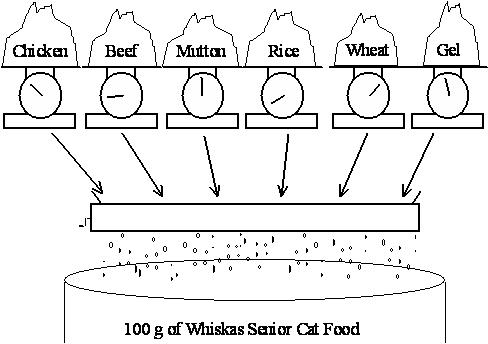
\includegraphics[scale=0.6]{images/whiskas_blend.jpg} 
\caption{The quantity of each ingredient must be determined.}
\end{figure}
The costs of the chicken, beef, and mutton are \$0.013, \$0.008 and \$0.010 respectively, while the costs of the rice, wheat and gel are \$0.002, \$0.005 and \$0.001 respectively. (All costs are per gram.) For this exercise we will ignore the vitamin and mineral ingredients. (Any costs for these are likely to be very small anyway.) 
Each ingredient contributes to the total weight of protein, fat, fibre and salt in the final product which must be 100g (very convenient). The contributions (in grams) per gram of ingredient are given in the table below. 

\begin{table}
\centering
\begin{tabular}{|l|l|l|l|l|}\hline
 		& Protein & Fat   & Fibre & Salt\\\hline
Chicken 	& 0.100 & 0.080   & 0.001 & 0.002\\
Beef 		& 0.200 & 0.100   & 0.005 & 0.005\\
Rice 		& 0.000 & 0.010   & 0.100 & 0.008\\
Wheat bran 	& 0.040 & 0.010   & 0.150 & 0.000\\\hline
\end{tabular}
\caption{Table of ingredient compositions.}
\end{table}

A Linear Program consists of three main parts. These are the variable definitions, the objective function and the constraints.

\subsubsection{Variable definition}
In this problem the variables will be defined as the quantity (in grams) of each ingredient to include in the can. These variables will be continuous and will be able to take any non-negative value. Mathematically, we define set $I$ as the set of ingredients then create an $x$ variable indexed by $I$

\begin{eqnarray*}
I &=& \{chicken, beef, mutton, rice, wheat, gel\}\\
x_i &\ge& 0 \quad \quad i \in I.
\end{eqnarray*}

\lstinputlisting[linerange={4-12}]{code/whiskas.py}

\subsubsection{Objective Function}
The objective function is to minimise the cost of production for each can.
\[
\min \sum_i c_i x_i.
\]
Where:
\begin{itemize}
 \item $c_i$ is the cost per gram of ingredient $i$.
\end{itemize}

\lstinputlisting[linerange={14-17}]{code/whiskas.py}

\subsubsection{Constraints}
Constraints serve to control the total mass of the ingredients and to model the protein, fat, salt and fibre requirements.

\begin{align*}
\sum_i x_i &= 100 \; \text{\hspace{19 mm}can mass} \\
\sum_i p_i x_i &\ge 8.0   \; \text{\hspace{20 mm}protein} \\ 
\sum_i f_i x_i &\ge 6.0   \; \text{\hspace{20 mm}fat} \\
\sum_i b_i x_i &\le 2.0   \; \text{\hspace{20 mm}fibre} \\
\sum_i s_i x_i &\le 0.4   \; \text{\hspace{20 mm}salt}.  
\end{align*}
Where:
\begin{itemize}
 \item $p_i$ is the protein per gram of ingredient $i$;
 \item $f_i$ is the fat per gram of ingredient $i$;
 \item $b_i$ is the fibre per gram of ingredient $i$;
 \item $s_i$ is the salt per gram of ingredient $i$.
\end{itemize}

\lstinputlisting[linerange={18-29}]{code/whiskas.py}

The pulp model must now be solved with some third party optimisation software. 
Pulp currently supports solving with coin-or \cite{coin-or}, glpk \cite{glpk}, 
CPLEX \cite{cplex} and Gurobi \cite{gurobi}.
The pulp download includes compiled versions of the coin-or solver for ubuntu and windows computers.

\lstinputlisting[linerange={31-37}]{code/whiskas.py}

\section{Other Example LP models}

Modelling the diet problem is not the only application of linear programming. Other examples include:
\begin{itemize}
 \item the transportation problem,
 \item the set partitioning problem,
 \item the assignment problem,
 \item the knapsack problem.
\end{itemize}
In this section we will give short examples of the first two problems modelled in pulp together with a brief description.

\subsection{The Transportation Problem (beerdistribution.py)}
A transportation problem involves that shipment of items from a set of sources 
to a set of sinks (the sources and sinks must be disjoint sets), the problem seeks 
to minimise the cost of shipping. In this case-study 
crates of beer must be shipped from two breweries to five bars.

\begin{figure}[h]
 \centering
 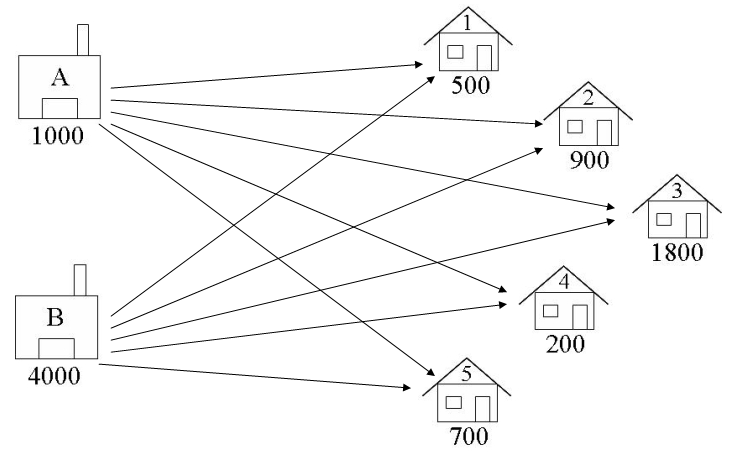
\includegraphics[scale = 0.3]{images/beerdistribution.png}
 \caption{The brewery and bar capacities and possible routes.}
\end{figure}


The problem is created.
\lstinputlisting[linerange={37-38}]{code/beerdistribution.py}

A list of possible routes for transportation is created:
\lstinputlisting[linerange={40-41}]{code/beerdistribution.py}

The variables created determine the amount shipped on each route. The variables
are defined as \lstinline{pulp.LpInteger} therefore solutions must not
ship fractional numbers of crates.
\lstinputlisting[linerange={43-47}]{code/beerdistribution.py}

The objective is to minimise the total shipping cost of the solution.
\lstinputlisting[linerange={48-50}]{code/beerdistribution.py}

These constraints ensure that amount shipped from each brewery is less 
than the supply available. The names given to the constraints will be preserved
when an `.lp' file is created.
\lstinputlisting[linerange={52-55}]{code/beerdistribution.py}

These constraints ensure that amount shipped to each bar is greater 
than the demand of the bar. These could also be equality constraints, depending 
on how the problem is modelled.
\lstinputlisting[linerange={57-60}]{code/beerdistribution.py}

\subsection{The Set Partitioning Problem (wedding.py)}
A set partitioning problem determines how the items in one set (S) can be partitioned into smaller 
subsets. All items in S must be contained in one and only one partition. Related problems are:
\begin{itemize}
 \item set packing - all items must be contained in zero or one partitions;
 \item set covering - all items must be contained in at least one partition.
\end{itemize}
In this case study a wedding planner must determine guest seating 
allocations for 
a wedding. To model this problem the tables are modelled as the partitions and the guests invited to the wedding
are modelled as the elements of S. The wedding planner wishes to maximise the total happiness of all of the tables. 

A set partitioning problem may be modelled by explicitly enumerating each 
possible subset. Though this approach does become intractable for large numbers of items (without using
column generation \cite{columngeneration}) it does have the advantage that the objective function co-efficients for
the partitions can be non-linear expressions (like happiness) and still allow this problem to be solved
using Linear Programming.

First we use \lstinline{pulp.allcombinations} to generate a list of all possible table seatings.
\lstinputlisting[linerange={20-22}]{code/wedding.py}

Then we create a binary variable that will be 1 if the table will be in the solution, or zero otherwise.
\lstinputlisting[linerange={24-28}]{code/wedding.py}

We create the \lstinline{LpProblem} and then make the objective function. Note that
happiness function used in this script would be difficult to model in any other way.
\lstinputlisting[linerange={30-32}]{code/wedding.py}

We specify the total number of tables allowed in the solution.
\lstinputlisting[linerange={34-35}]{code/wedding.py}

This set of constraints defines the set partitioning problem by guaranteeing that a guest is allocated to
exactly one table.
\lstinputlisting[linerange={38-41}]{code/wedding.py}



\section{Why pulp}
Modelling problems using LP and solving them with pulp can be a very useful approach for the python programmer. 
This approach allows the programmer to focus on the modelling rather than the algorithms that find the solution.
The third party LP solvers that pulp interfaces with are all mature pieces of software that can be trusted to 
produce the correct solution to the model created in pulp. The difference between these solvers, for a user of pulp, 
lies mainly in the trade off between cost of the solver and its speed to find a solution.

LP and IP are well researched areas of mathematics, therefore once a problem is stated as an LP model it is possible 
to guarantee some properties of the solutions given. For instance, if the solver delivers an optimal solution it 
will be impossible for someone to create a solution that is better (as measured by the objective function).

Compared to other LP modelling tools including AMPL \cite{ampl}, GAMS \cite{gams}, mathprog \cite{glpk}, flopc++ \cite{flopc}, and pyomo \cite{pyomo} and poams; pulp offers a number of advantages. These include its:
\begin{itemize}
\item  non-restrictive licensing;
\item  ease of installation;
\item  clear syntax;
\item  interoperability with an number of solvers;
\item  extensive documentation.
\end{itemize}

\subsection{Licensing}
The licensing of pulp under a permissive open-source license allows pulp to be used as a medium for teaching
operations research as students can download and use pulp for free. The license allows OR practitioners to 
integrate pulp in commercial applications for their clients without disclosing how the problem was solved. 
The license also allows advanced users to modify and improve pulp for their own purposes.

\subsection{Installation}
Pulp is very easy to install. The provision of a setup.py file and registration on pipy, allows the user
to use
\begin{verbatim}
 $easy_install pulp-or
\end{verbatim}
to download and install pulp on their system. For windows and ubuntu users this binary package also includes
the coin-or \cite{coin-or} solver so pulp will be immediately functional. For users on other platforms a compatible 
solver must be installed for a pulp model to be solved.

\subsection{Syntax}
Ideally an LP modelling framework will allow a one-to-one translation of symbols from mathematical notation. If the syntax follows the formulation the programmer can ensure that the model written is the model required. The OR practitioner can also quickly read and understand the a model as written pulp, without having much python background. The standard mathematical notation is very concise  and therefore code that mimics it will also be clear and concise.

The use of a `Pythonic' construction of the pulp framework allows the programmer to use it easily in a variety of ways. Pulp can be directly imported into the local name-space (against python style) to allow simple LP models to be written by non-programmers, in fact most of the case studies on the wiki \cite{pulpwiki} use this style. Pulp also does not force the programmer to use any particular way to store parameter data. Parameter data can be stored as lists, dictionaries or custom classes.

\subsection{Interoperability}
The ability for pulp to call a number of free and non-free solvers is important as the OR practitioner often wishes to compare the solution of a problem with a variety of solvers. The user may wish to develop simple LP models in a free solver and then provide a solution to a client using a commercial solver. The use of non-free solvers may dramatically reduce the solution time of the model. Pulp allows the free interchange of solvers without much change in the program, only a parameter for the \lstinline{LpProblem.solve} function is changed.

\subsection{Documentation}
Pulp is supplied with a user guide with extensive examples (in fact it was converted from a course teaching LP modelling). This user guide and the permissive license were intended to make pulp useful to the largest possible audience.

\section{Conclusion}
In conclusion pulp nicely bridges the gap between the OR practitioner and the python programmer. This allows the OR practitioner to use python to quickly develop and solve LP and IP models while having access to all of the tools available in the python standard library. The python programmer can now embed LP models in complex programs written in python. So next time you find yourself hacking up an algorithm to solve some problem in your code please consider if it would be appropriate to model this problem as an LP or IP instead. If so download and use pulp.

\section*{Appendix - Example Code in full}
\subsection*{whiskas.py}
\lstinputlisting{code/whiskas.py}

\subsection*{beerdistribution.py}
\lstinputlisting{code/beerdistribution.py}

\subsection*{wedding.py}
\lstinputlisting{code/wedding.py}


%------------------------------------------------------------------------- 
%--- back matter: bibliography ---
% These are in alphabetical by leading author order.
\newpage
\bibliographystyle{IEEEtran}
\bibliography{references}
%------------------------------------------------------------------------- 
% We need this for the style to work properly, so please leave it in here:
\label{lastpagenum}
\end{document}
